\documentclass[osajnl,twocolumn,showpacs,superscriptaddress,10pt]{revtex4-1}


%PAQUETES<<<<<<<<<<<<<<<<<<<<<<<<<<<<<<<INICIO
\usepackage{dcolumn}% Align table %columns on decimal point
\usepackage{bm}% bold math
%
%Paquete de Idioma
\usepackage[spanish]{babel}
%
%Codificación Alfabeto
\usepackage[utf8]{inputenc}
%
%Codificación de Fuente
\usepackage[T1]{fontenc}
%
%Índice
\usepackage{makeidx}
%
%Gráficos3
\usepackage{graphicx}
\usepackage{subfig}
% \usepackage{longtable}
%\usepackage{xcolor} 
%
%Matemática
\usepackage{amsmath}
\usepackage{amsfonts}
\usepackage{amssymb}
%\usepackage{amstext} 
%
%Estilo de Página Numeración superior
%\pagestyle{headings}
%
%Hiperlinks \href{url}{text}
\usepackage[pdftex]{hyperref}
%
%Graficos y tablas
\usepackage{multirow}
%\usepackage{multicol}
\usepackage{float}
\usepackage{booktabs}
%
\decimalpoint
%\bibliographystyle{IEEEtran}
%\bibliography{IEEEabrv,mybibfile}
%
%
%PAQUETES<<<<<<<<<<<<<<<<<<<<<<<<<<<<<<<INICIO

\begin{document}
%SIGNOS
%TILDE -> \' <vocal>
%TEXTO_NEGRITA -> \textbf{<texto>}
%TEXTO_ITALICA -> \textit{<texto>}
%TEXTO_SUBRAYADO -> \underline{<texto>}

%TITTULO DEL ARTICULO
\title{\Huge IoT Práctica Uno -  Buzón Inteligente - Arquitectura de Computadores y Ensambladores 2 }
%AUTORES DEL ARTICULO

\author{\newline Airton Yelstin de León Obando (201602836) - Rol: Analítico}
\affiliation{Grupo No.7 - Universidad de San Carlos de Guatemala, Escuela de Ciencias y Sistemas
}%

\author{\newline Edgar Mauricio Gómez Flores, (201114340) Rol: Infraestructura del Producto}%
\affiliation{Grupo No.7 - Universidad de San Carlos de Guatemala, Escuela de Ciencias y Sistemas
}%
\author{\newline Jurgen Andoni Ramirez Ramirez, (201404179) Rol: Conectividad}%
\affiliation{Grupo No.7 - Universidad de San Carlos de Guatemala, Escuela de Ciencias y Sistemas
}%
\author{\newline Josue Eduardo Abelarde Perez, (201602890) Rol: Smart-APP}%
\affiliation{Grupo No.7 - Universidad de San Carlos de Guatemala, Escuela de Ciencias y Sistemas
}%
\date{Agosto 2020}



%INICIO DE DOCUMENTO<<<<<<<<<<<<<<<<<<<<<<<<<<<<<<<<<
\begin{abstract}
\title {resumen}
En esta pr\'actica se pretende hacer uso del concepto de Internet de las Cosas ( IoT - Internet of Things ) aplicado a un buz\'on de correo inteligente. Este buz\'on se diseño de tal forma que sea capaz de transmitir informaci\'on de manera inmediata del estado de este mismo al usuario final, lo anterior por medio de diferentes dispositivos electrónicos y sensores, adem\'as de un microcontrolador ARDUINO que recolecta la informaci\'on y la transmite a la nube. Todo lo anterior de manera que el usuario final tiene informaci\'on actualizada de su buz\'on desde su dispositivo m\'ovil en cualquier momento y lugar.
\end{abstract}
\maketitle{}
\section{INTRODUCCIÓN}
Al hablar de introducir el concepto de IoT es este proyecto principalmente se habla de la importancia de recolectar datos y hacer uso de estos datos provenientes de cualquier objeto de la vida diaria cuya utilidad aumenta significativamente al convertir estos datos en información relevante y de interés en su funcionamiento, de tal manera que este objeto expande sus funciones para las que fue originalmente creado. Este buzón inteligente fue diseñado para proveer una solución a los problemas de sanidad e higiene ante los acontecimientos de la pandemia del nuevo virus SARS-COVID19. Debido a lo anterior este buzón inteligente es capaz de desinfectar paquetes entregados al domicilio del usuario de manera automática para prevenir la propagación de la enfermedad, esto gracias a un rociador con una sustancia desinfectante y gracias a un conjunto de diferentes dispositivos y sensores instalados que funcionarán en conjunto, el buzón inteligente tiene la capacidad obtener el estado de las puertas del compartimiento y el usuario podrá saber en todo momento el estado de su buzón, además no solo podrá saber cuando un nuevo paquete haya sido introducido sino también podrá saber los niveles del liquido desinfectante en el recipiente para prevenir que este se agote y todo desde su dispositivo móvil desde cualquier lugar y en cualquier momento. La comunicación es posible a través de una aplicación para dispositivos móviles con conexión a internet e información proveniente la nube.

\section{Prototipo de Diseño}
Considerando que el propósito de este objeto es para introducir paquetes y resguardarlos se presentan los prototipos de diseño utilizados para la realización del buzón inteligente, observar Figura 1.


\begin{figure} [H] \centering 
\caption{Boceto de diseño}

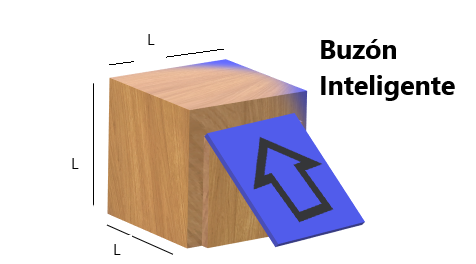
\includegraphics[width=0.5\textwidth]{Boceto.png} 
Las dimensiones son de L = 30 cm de alto, ancho y largo con una puertecilla móvil para introducir los paquetes.
\end{figure}

\section{Famework de Productos Inteligentes Conectados}
\subsection{Infraestructura del Producto}
\subsubsection{Hardware:}
\begin{itemize}
    \item[$\bullet$]\textbf{Maqueta} para buzón inteligente.
    \item[$\bullet$]\textbf{Rociador o atomizador} para la desinfección de paquetes.
    \item[$\bullet$]Dispositivo de \textbf{Módulo WiFi}.
    \item[$\bullet$]\textbf{Arduino.}
    \item[$\bullet$]\textbf{Cables} para conexiones.
    \item[$\bullet$]\textbf{Cautín} para realizar soldaduras.
    \item[$\bullet$]\textbf{Estaño.}
    \item[$\bullet$]\textbf{Protoboard} para armar circuitos digitales.
    \item[$\bullet$]\textbf{Módulo Magentico Tipo Reed} para comprobar el estado de las puertas
    \item[$\bullet$]\textbf{Bomba dispensadora} para accionar rociador de desinfectante.
    \item[$\bullet$]\textbf{Recipiente contenedor} de desinfectante, este contenedor es de plástico.
\end{itemize}
\subsubsection{Software}
    Se han diseñado y programado los algoritmos para la recolección de datos sobre el estado del buzón en el microcontrolador ARDUINO para su posterior trasmisión a la nube.
    
\subsection{Sensores}
\begin{itemize}
    \item[$\bullet$]\textbf{Sensor de peso} para determinar la presencia de nuevos paquetes.
    \item[$\bullet$]\textbf{Sensor ultrasónico HC-SR04} para calcular la cantidad de sustancia desinfectante en el contenedor.
    \item[$\bullet$]\textbf{Sensor magnético tipo Reed} para determinar el estado de las puertas del buzon.
\end{itemize}
\subsection{Conexión}
    La comunicación a utilizar entre el buzón inteligente y el usuario será a través de conexión \textbf{WiFi}. El dispositivo arduino recolecta la información para ser transmitida desde el módulo \textbf{WiFi} realizando peticiones \textbf{HTTP} con el servidor a través de una \textbf{API/REST} que se encargará de transmitir la información al dispositivo móvil del usuario. Ver figura 2. \newline
\begin{figure} [H] \centering 
\caption{Representación de conexión}

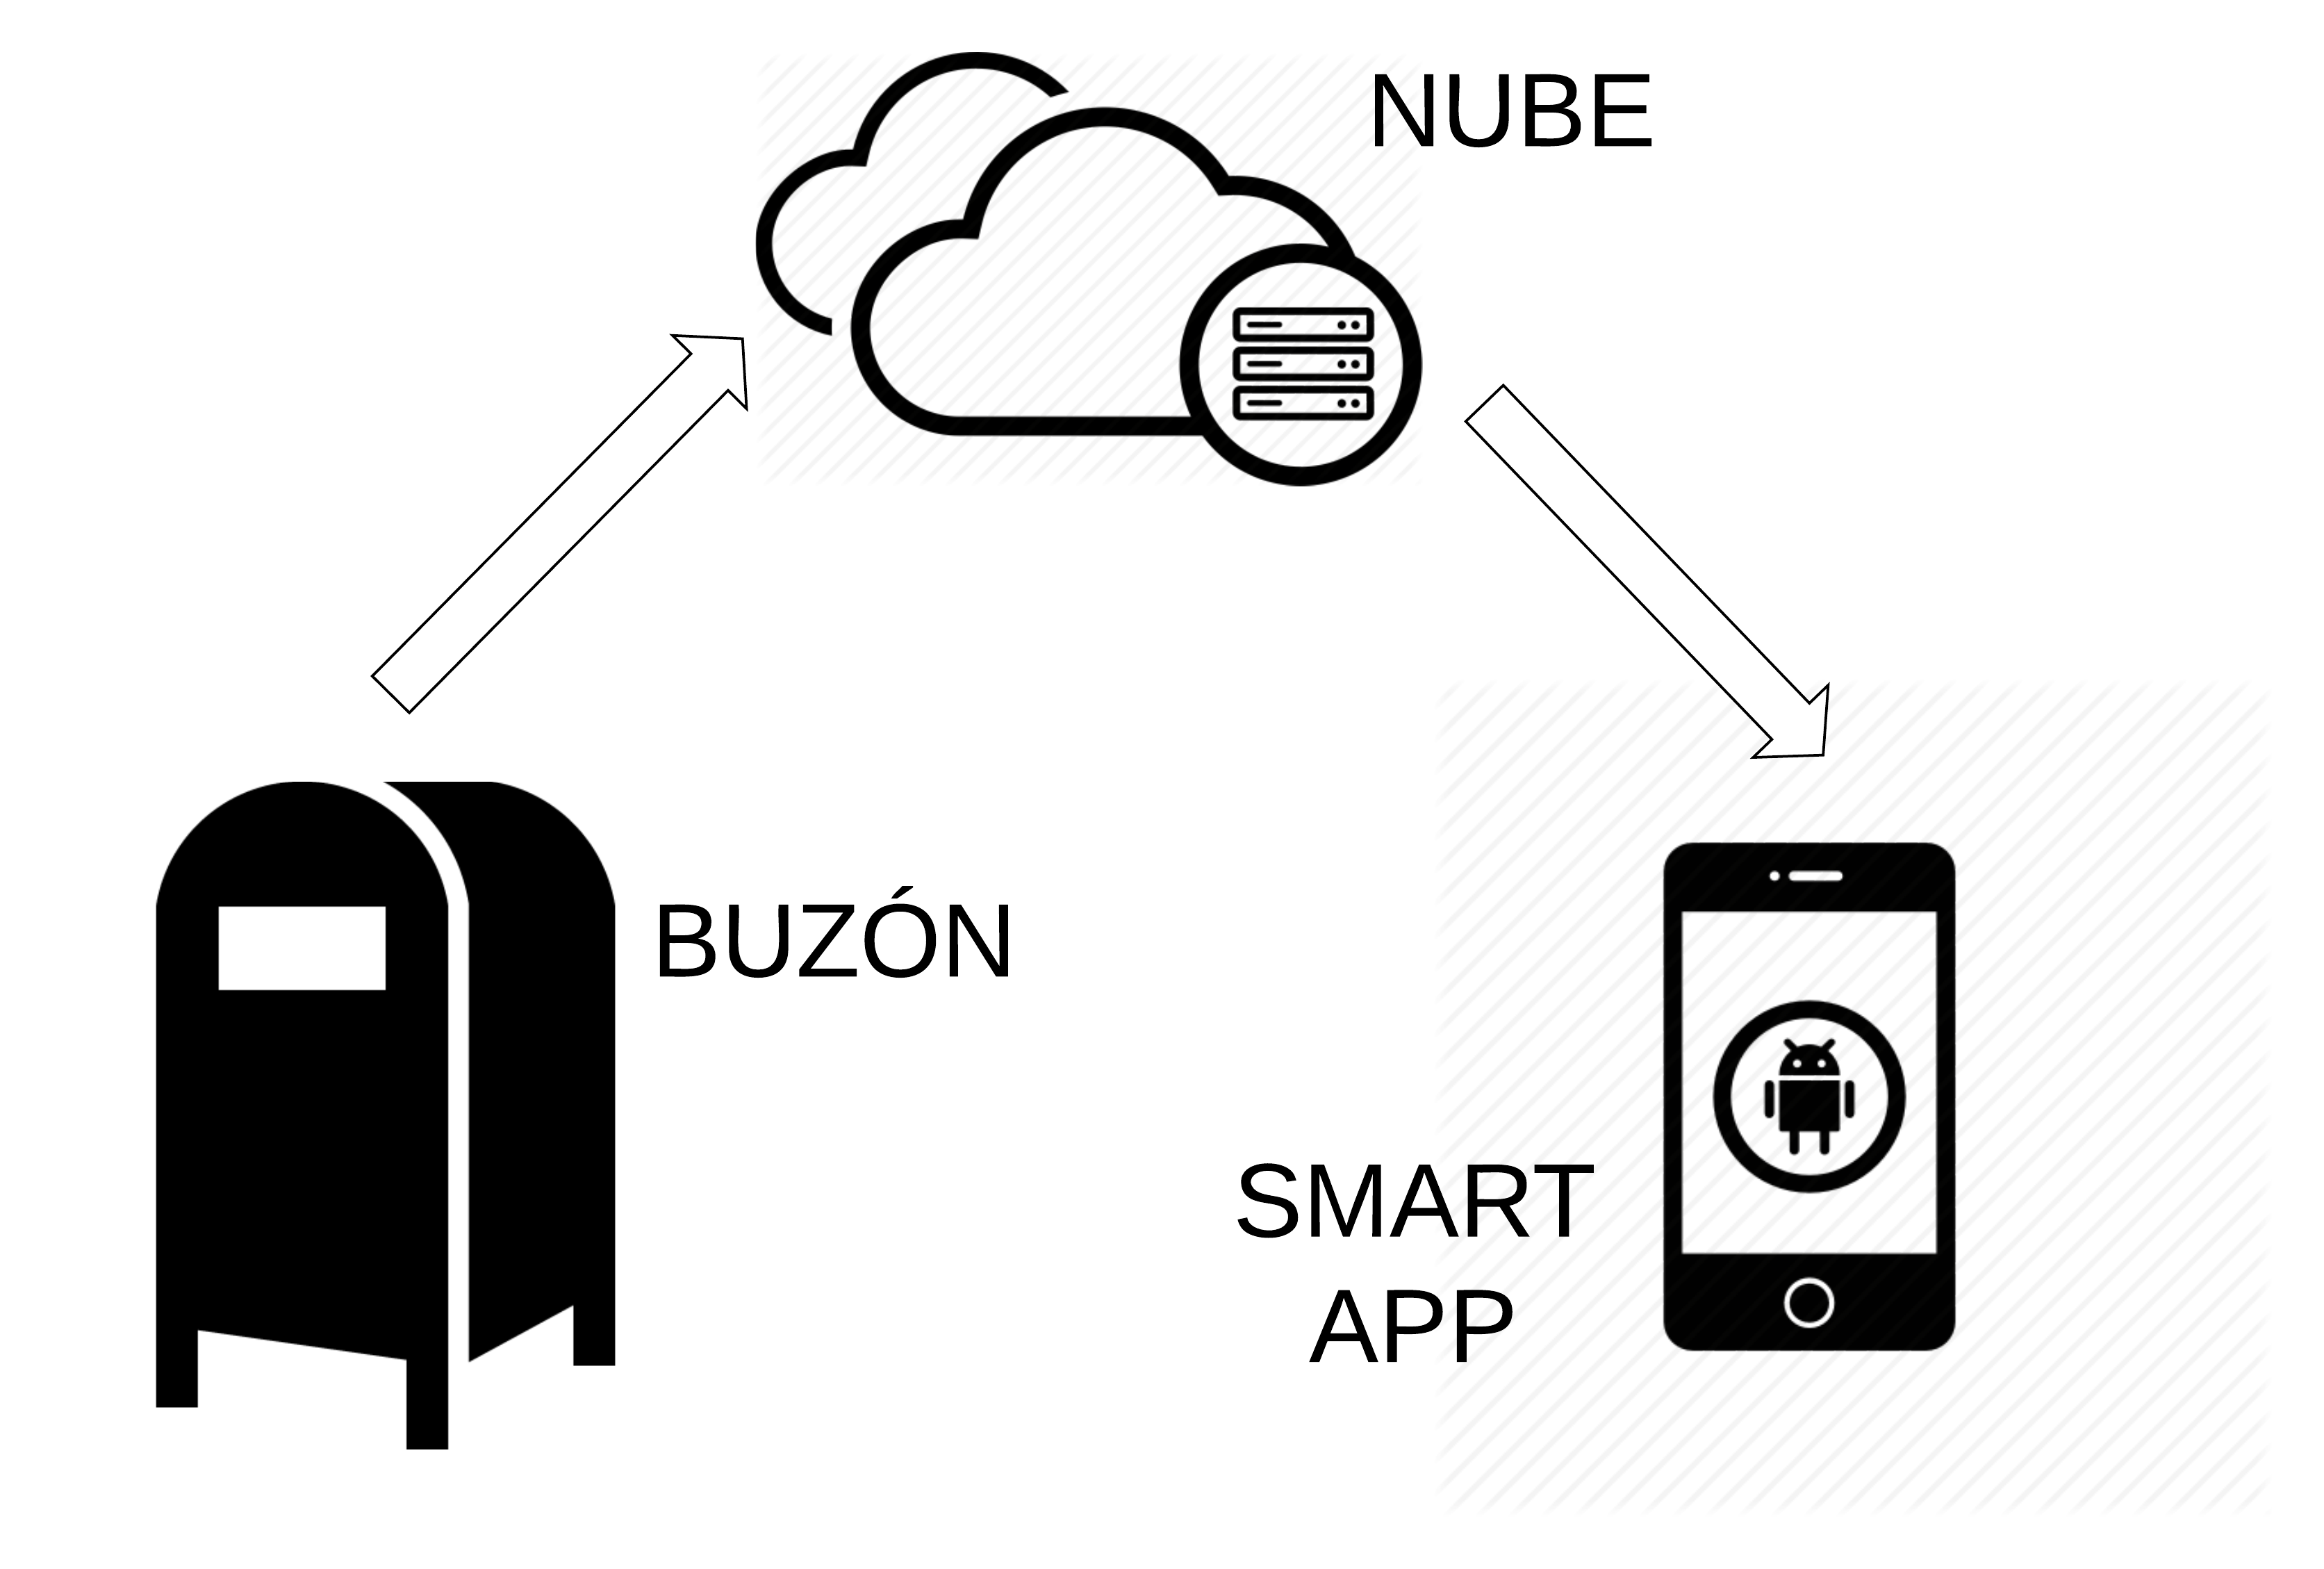
\includegraphics[width=0.5\textwidth]{conection.png} 
\end{figure}
\subsection{Análisis}
    Para este proyecto solamente se requiere que el buzón desinfecte los paquetes entregados una vez están dentro del compartimiento del buzón, además este producto de IoT debe informar al usuario sobre nuevos paquetes, estado de las puertas del buzón y nivel de líquido desinfectante y por lo tanto \textbf{no es necesario aplicar análisis en este proyecto.}
\subsection{Smart APP}
    Ya que el usuario deberá tener acceso al estado de su buzón inteligente en todo momento se ha de ha desarrollado una aplicación inteligente para dispositivos móviles. Esta aplicación es compatible con dispositivos que utilizan el Sistema Operativo \textbf{Android}, a continuación se pueden apreciar las pantallas que muestran su funcionamiento:
    
\begin{figure} [H] \centering 
\caption{PANTALLA 1 ( Aplicación móvil )}
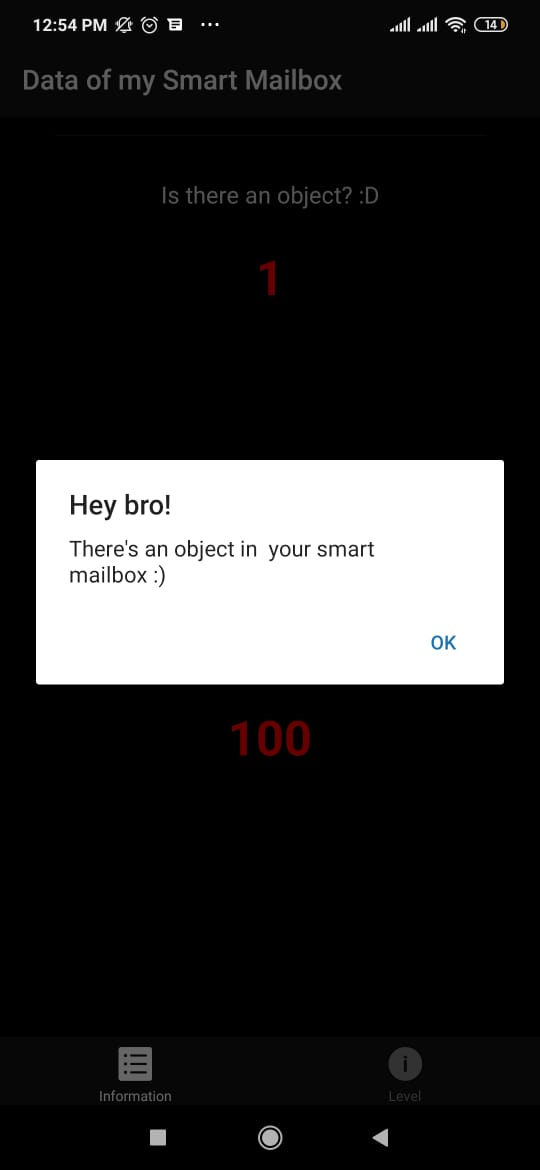
\includegraphics[width=0.4\textwidth]{img4.jpeg} 
\end{figure}
\\
Cuando el buzón ha detectado un nuevo paquete en el compartimiento la aplicación muestra una advertencia al usuario sobre ello. Al seleccionar vera más información sobre ello.

\begin{figure} [H] \centering 
\caption{PANTALLA 2 ( Aplicación móvil )}
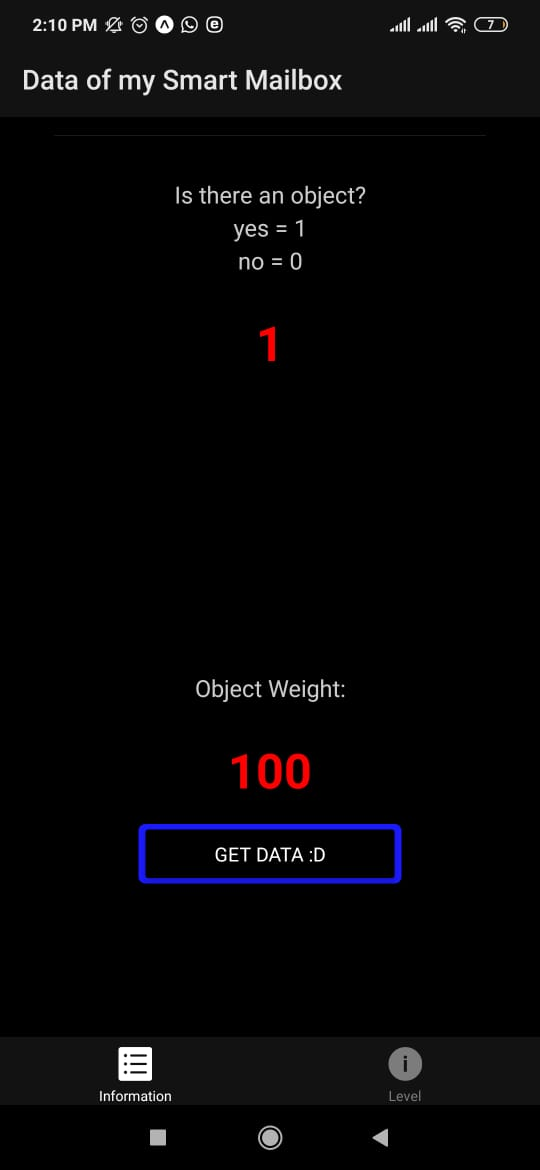
\includegraphics[width=0.4\textwidth]{img2.jpeg} 
\end{figure}
\\
Una vez el buzón inteligente ha reconocido que se ha introducido un nuevo paquete la aplicación actualizara su estatus en la pantalla principal indicando la información de interés. Si hay un objeto mostrará un número uno de lo contrarios un número cero, además el peso del objeto y si se desea ver más solo debe presionar el botón \textbf{Get Data}.

\begin{figure} [H] \centering 
\caption{PANTALLA 3 ( Aplicación móvil )}
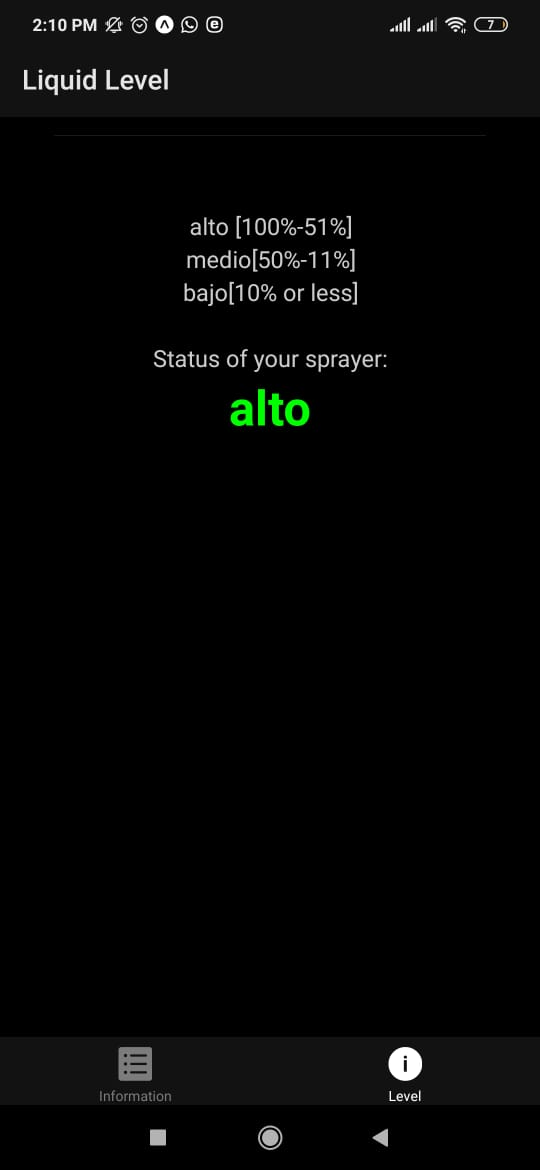
\includegraphics[width=0.4\textwidth]{img3.jpeg} 
\end{figure}
\\
Una vez se ha presionado el botón \textbf{Get Data}  el usuario puede ver la información detallada junto con el nivel de liquido desinfectante.

\section{Vídeos de funcionamiento}
\begin{itemize}
    \item[$\bullet$]Video1: https://youtu.be/1RXLjeAWD9k 
    \item[$\bullet$]Video2: https://youtu.be/fiz1PkFIdJ8
    \item[$\bullet$]Video3: https://youtu.be/uYKBNuGgTSc
\end{itemize}





\end{document}
